\documentclass[10pt, letterpaper, twoside]{article}

\usepackage{epsfig}
\usepackage{verbatim}

\pagestyle{headings}     

\author{Tania Bedrax-Weiss \and Conor McGann \and Andrew Bachmann \and Will Edgington \and Michael Iatauro \\
QSS Group Inc. \\
Computational Sciences Division \\
NASA Ames Research Center \\
Moffett Field, CA 94034-1000 \\
\{tania,mcgann,bachmann,wedignt,miatauro\}@email.arc.nasa.gov
}

\title{\ET: User Guide}

\begin{document}

\newcommand{\ET}{EUROPA\,2}

\maketitle

\tableofcontents

\section{Introduction}
\ET\, is the next generation of the Extensible Universal Remote
Operations Architecture.  Like the CLARATy robotics control architecture
\cite{kn:Ne}, MDS \cite{MDS}, or ILOG \cite{ILOG}, \ET\, is a
component-based software library for representation and reasoning with
plans and schedules. Our goal in developing \ET\, is to provide a fast,
flexible, extensible, reusable technology platform for building planning
and scheduling applications suitable for space exploration.

EUROPA \cite{caip,plan} which has been the core planning technology for a
variety of NASA-relevant research and mission applications. A notable
example is MAPGEN \cite{mapgen}, the ground-based daily activity planning
system for the Mars Exploration Rover mission. EUROPA in turn is derived
from HSTS which was the planner for the Remote Agent\cite{ra}. \ET\,
builds on the legacies of EUROPA and HSTS and provides improvements in
performance, expressivity, reasoning capabilities, flexibility,
extensibility, and modularity which has opened the technology to a broader
range of planning techniques (e.g. POCL planning).

\subsection{Plan Services}
\ET\, provides the following services:
\begin{itemize}
\item Domain modeling: for describing planning domains
\item Plan representation: for updating partial plans 
\item Constraint propagation: for propagating the consequences of updates
to plans and determining violations
\item Subgoaling: for generating consequences of commitments in the plan
\item Flaw definition: for specifying flaws from a partial plan
\item Decision management: for generating and resolving flaws
\item Plan assessment: for determining plan completeness
\end{itemize}
\ET\, provides the New Domain Description Language NDDL, which deviates
substantially from DDL in that it provides an object oriented syntax.  It
is also compiled, instead of interpreted.  NDDL provides syntax for
describing objects, timelines, resources, predicates, rules, variables, and
constraints. It also provides facilities like inheritance and containment
to describe complex objects.  Please see Section~\ref{nddl} for more
information on NDDL. 

Plan representation is a service provided by the Plan Database, much as it
was in EUROPA.  The Plan Database responds to plan modification operations
by updating the partial plan or invoking specialized components to update
parts of the partial plan.  Constraint propagation, for instance, is a
service provided by the Constraint Engine and is in charge of responding to
updates to constraints and variables triggered by the plan modification
operations. The Rules Engine is in charge of subgoaling also in response to
plan modification operations. 

Flaw definition, decision management, and plan assesment services are
provided by the CBPlanner module. The CBPlanner module implements a
chronological backtracking planner that resolves all flaws in the partial
plan except for temporal variable assignments as described in
\cite{planid,e2}. 

The philosophy underlying \ET\, is to acknowledge up front that no
one size fits all when it comes to which techniques to use, and which
capabilities to employ. Consequently, \ET\, is engineered to allow
people to take just what they need, discard what they do not, and
integrate extensions to suit their particular requirements in a
straighforward manner. The design strategy is to focus on a core
framework defininig the principal abstractions and interactions
induced by our underlying paradigm. We then provide concrete
components to allow particular assemblies to be defined. 

\subsection{\ET\, Design Goals}
To meet the needs of missions and research projects, the design of 
\ET\, must be: 1. Efficient to ensure low latency for operations and
queries; 2. Flexibile to ensure services can be selected and flexibly
integrated; 3. Extensible to ensure services can be enhanced to meet the
needs of research or mission applications. 

\subsubsection{Efficiency} \ET\, has produced significant gains in speed over
EUROPA. The primary contributors to the improvement arise from: 1. Fast
interfaces and specialized implementations: the ability to tune
implementations using inheritance provides speed improvements in key areas
such as operations on domains.  2. Efficient merging: \ET\, provides an
algorithm to handle merging operations that disables redundant constraints
arising in the plan database. 3. Incremental relaxation: when relaxing a
variable, \ET\, relaxes only variables reachable through the constraint graph.
4. Direct support for static facts: \ET\, uses objects to capture static
facts. Objects can be referenced through variables.  We provide a pattern
for existentially quantifying objects. By contrast, EUROPA used
timelines with a single predicate to capture this information, incurring a
high overhead through inefficient merging. 

\subsubsection{Flexibility} \ET\, is highly customizable. Support for
resources may be ommitted if a problem does not require resources. If a 
problem does not require compatibilities (e.g. a scheduling problem), the
rules engine can be omitted. If temporal constraints are not important in a
problem, the temporal propagator may be removed and/or replaced with the
default propagator. Only required constraints need to be registered. This
form of customization is useful as it allows systems to avoid incurring
costs for components that are not required. \ET\, also provides a language to
customize the system for new domain models.  Furthermore, heuristic and flaw
specifications are also provided. An open API ensures flexbility in how \ET\,
is integrated.

\subsubsection{Extensibility} \ET\, is highly extensible. As new problems are
encountered, or new algorithms are developed, there are many ways to
integrate new capabilities as specialized components e.g. constraints,
propagators, resources. This is essential for success in research and
mission deployments. 

The content of this guide is laid out as follows. We begin with an
explanation of the concepts underlying \ET\, addressing its role as
an embedded technology within a planner, and its underlying paradigms
for representation and reasoning. We then switch gears to get the
reader up and running with a particular assembly of \ET\, that is
included with the distribution. In this section, the reader will solve
a prepared planning problem with \ET, without really understanding
much about how it happened! Following this, we seek to build up some
understanding with a tutorial-like exposition of model development,
and problem solving with \ET's primary modeling language -
NDDL. Having spent some effort working on the application of \ET,
we turn to its underlying architecture. This section gets
'under-the-hood' to provide an understanding of how \ET\, works at
the implementation level.  Finally, we address the technical aspects
of customization and extension. Detailed reference material is
included in the appendices.

\section{Concepts}

\subsection{Plans in Planning, Scheduling and Execution}
Consider the scenarios illustrated in Figure \ref{Applications}. The first
is an application of automated planning where the input planning problem is
solved by a {\em Planner} to produce an acceptable partial plan. The role
of the {\em Planner} is to perform the search steps for resolving
flaws. Thus it interacts with a partial plan by imposing and retracting
restrictions. All operations are made on the {\em Plan Database} which
stores the partial plan.  The second is an application of automated
planning in concert with a {\em User}. The User may introduce goals into a
plan, and change or undo decisions previously made by a
Planner. Additionally, a User may employ a Planner to work on the current
partial plan.  In this case, changes are also made in response to queries
and operations on the {\em Plan Database}.  In the last figure, planning
technology is deployed for plan execution. A partial plan may be used by an
{\em Executive} for execution. In such a scenario, the partial plan is
updated throughout execution. The Executive may employ incomplete search to
refine the partial plan as it goes. A Planner may be employed to repair a
plan or develop a refinement of the plan as the mission progresses. In each
of the cases described, {\em clients} (i.e. Planner, User, Executive)
leverage the services of a common {\em server}, the {\em Plan Database}.
\begin{figure*}[t]
\centering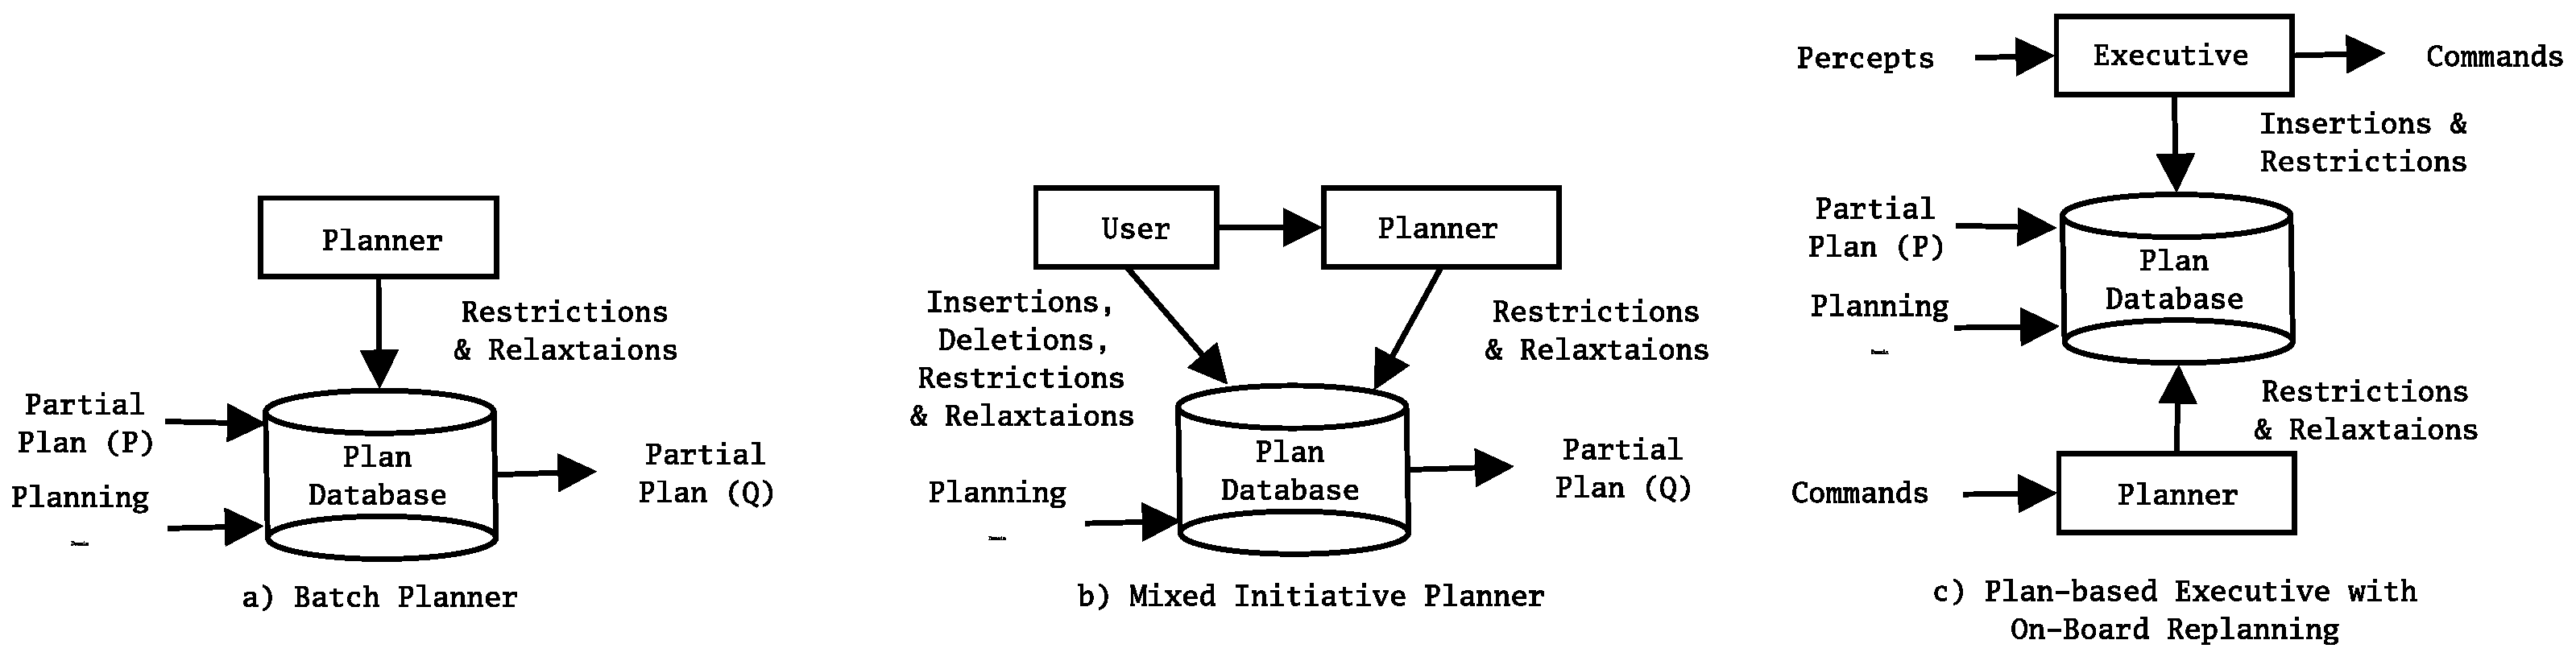
\epsfig{file=Applications.eps, width = 6.25in}
\caption{Sample Plan Database Applications}
\label{Applications}
\end{figure*}

\subsection{Model-Based Planning}
A {\em Model} expresses laws that govern a particular domain of interest.
A model for \ET\, usually contains descriptions of entities in the system
and relationships between them, that allow a planner/scheduler to infer
conditions that must be satisfied in order to arrive to a solution to a
problem based on that model.  Domains and problem instances are
described in \ET\, in NDDL.  A typical NDDL description will contain a set
of classes, predicates, and configuration rules.  Classes represent
properties of the world that may or may not evolve over time; predicates
(with variables) represent state descriptions; and configuration rules
represent relationships between state descriptions that must hold (the laws
of the domain). 

\subsection{Partial Plans: States and Relationships}
A {\em Partial Plan} represents a set of networks of states typically
ordered by time, though it can be ordered by precedence constraints or
completely unordered (e.g. a bag of states) in planning, scheduling, and
execution. Each network is represented as an {\em Object}, which
corresponds to an instance of a model class.  Objects that impose
mutual exclusions as well as a total order on its set of states is defined
as a {\em Timeline}. Objects that track numeric change are defined as
{\em Resources}.  Objects that are just bags of states are called
Objects. \ET\, provides means to specialize object implementations.

States in Objects are represented by {\em Tokens} and can correspond to
activities in scheduling, actions and fluents in planning, and commands in
execution. Tokens are instances of predicates, and like predicates, they
contain variables that can be used to augment state descriptions. Some of
these variables can be temporal variables indicating the temporal extent of
the token/state.  Relationships among tokens are defined by configuration
rules.  Configuration rules specify relationships among tokens (e.g.
subgoaling relationships) expressed as constraints between variables of
tokens.

\subsection{Token State Model}
A token in \ET\, evolves as decisions are made.  Initially a token may be
{\em active} or {\em inactive.  A token is {\em active} if commitment to
the token being in the plan is made.  A token is {\em inactive} otherwise. 
All token flaws that can be inferred from the partial plan and the model
via configuration rules are represented as {\em Inactive Tokens}. Figure
\ref{TokenStateTransition} illustrates the states and transitions of tokens
in \ET. A token is {\em Active} immediately when introduced by an actor
external to the plan database, as is the case with a goal $G$ specified in
an initial partial plan. A token is initially {\em Inactive} when
introduced by a configuration rule of the predicate of an {\em Active
Token}.  As prescribed by CAPR \cite{e2}, an inactive token corresponds to
a token flaw which can be resolved by either {\em merging} with a matching
{\em Active Token} or by choosing to use the resolver $\top$ via {\em
activation}. Merging is chosen to represent that the configuration rule is
satisfied by an existing state, that which is active and participates in
merging. Activation is chosen to represent that a new state is needed to
satisfy the configuration rule. 
\begin{figure}[t]
\centering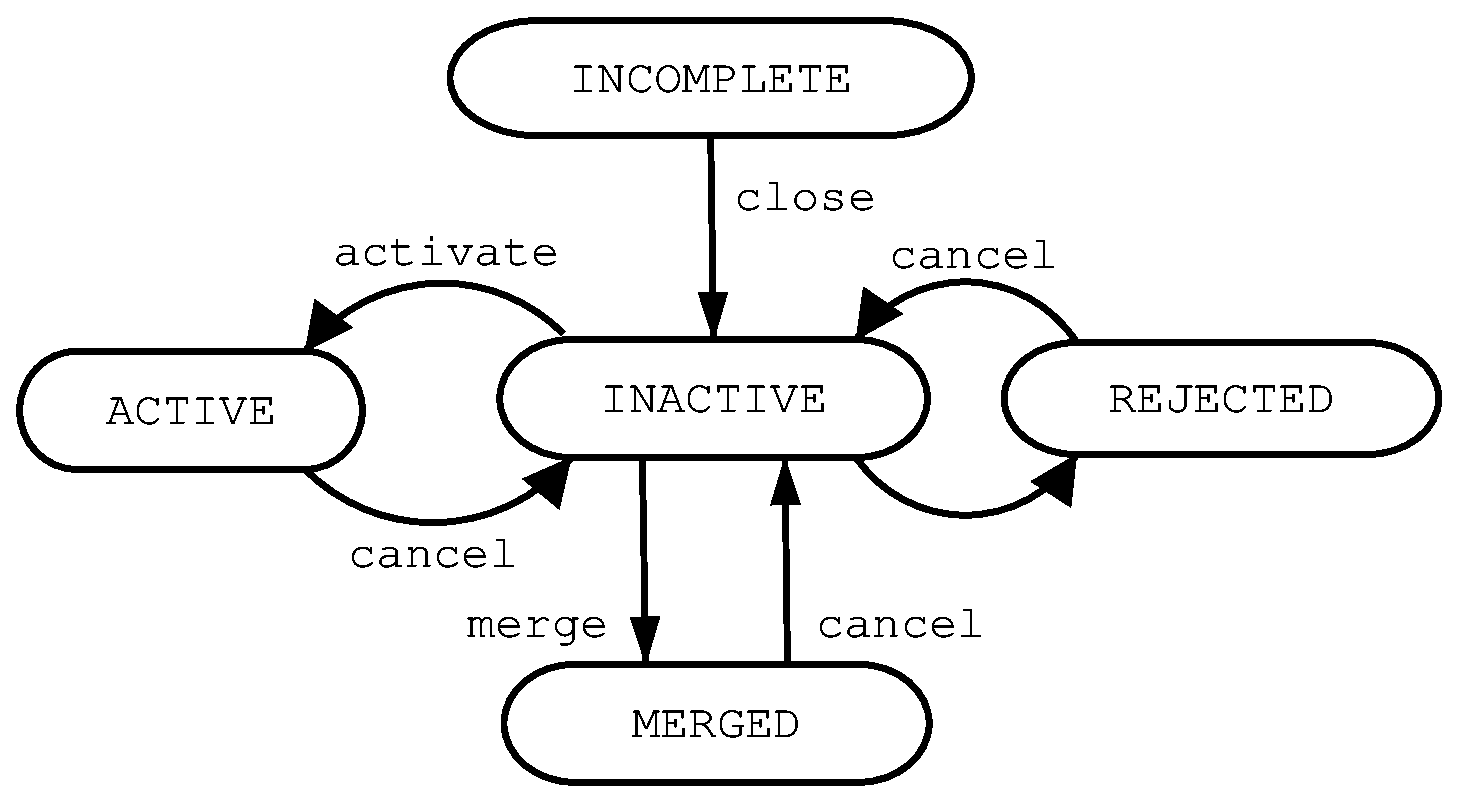
\epsfig{file=TokenStateModel.eps, width = 3.25in}
\caption{Token State Transition Diagram}
\label{TokenStateTransition}
\end{figure}

\subsection{Planning/Scheduling Decisions}
Planning/scheduling decisions arise from flaws in the partial plan.  Flaws
can be either unsatisfied configuration rules, unordered tokens in objects
(if they have specific ordering requirements), or unbound variable
assignments.  A planner is done when it has verified that all applicable
configuration rules are satisfied.  A configuration rule is applicable when
there is an active token with a predicate that matches a configuration rule
in the model.  Unbound variables may occur in tokens, objects, or rules.
These must be bound to singletons before the planner can deem the plan
complete.  There are a few caveats, however.  \ET\, provides the ability to
plan within a specific horizon.  Thus, tokens and variables of tokens that
lie outside of the horizon will not be deemed as flaws.  By default, the
horizon is [-INFINITY, +INFINITY], but the horizon may be specified in the
initial state. Another caveat is that we provide a mechanism for specifying
precisely the set of flaws that should be resolved before the planner
finishes ``completing'' the partial plan.  This mechanism is explained in
full in a paper \cite{planid}, however, we mention that flaws can be
included in the set that need to be resolved via the specification of
conditions that flaws must satisfy.  Thus, a plan is not complete until all
flaws that satisfy all conditions are resolved.

\subsection{Early vs. Delayed Commitment}
\ET\, provides at ways of controlling early vs. delayed commitment through
controlling variable assignments.  One example is how \ET\, handles
temporal assignments.  \ET\, allows representation and reasoning over
temporal intervals.  This flexibility turns out to be very useful when
there's lack of knowledge on precisely when states will hold.  Temporal
variable assignments can be delayed indefinitely by excluding them from the
set of flaws.  This can be done via a mechanism we call Plan
Identification \cite{planid}.  In brief, \ET\, provides a set of standard
conditions that candidate flaws have to pass in order to become flaws that
must be resolved for planning to complete.  One of these conditions is a
temporal variable condition that filters out all temporal variables, thus,
temporal variables never appear as variables whose assignments need to be
made. 

Another way of controlling early vs. delayed commitment can be done by
specifying rules conditional on variable assignments.  A heuristic can then
be used to determine when such variable assignments should be made, and
when subgoaling can occur.

\section{Hello Rover - Getting started with PLASMA}

This section will demonstrate a simple example that takes an initial state
and a model and runs a planner on them to produce a plan.  \ET\, does not
include a GUI.  However, you can use an adjunct project called PlanWorks to
visualize a plan and step through the planning process once the planner has
produced a plan.  This section will illustrate how to get started with \ET.

\subsection{Creating a Project}
After successfully building \ET\, by following the instructions in the
README and BUILDING files located in the PLASMA root directory, you can
create your own project by invoking ``makeproject'' with the name of your
project as an argument in the PLASMA root directory.  This will create a
directory with the name of your project that is parallel to the PLASMA
directory.  In it you'll find the following files: Jamrules, Jamfile,
<Project>-Main.cc, <Project>-initial-state.nddl <Project>-model.nddl and
ppw-config.  \ET\, uses Jam instead of make to build its files.  Jamrules
and Jamfile are both part of the build system.  Jamrules specifies some
variables and establishes dependencies with \ET.  Jamfile specifies the
main program and its dependencies.  ppw-config is a file that contains
configuration options for PlanWorks.  PlanWorks is a plan visualization
system that can be installed along with \ET\, to aid in understanding and
debugging.  <Project>-initial-state.nddl contains the initial state or
problem description and <Project>-model.nddl contains the model or domain
description. Both files contain descriptions in the NDDL language.
Finally, the <Project>-main.cc contains the main program that creates an
assembly (configuration of \ET\, components) and plans based on the given
initial state and model files.

\subsection{Building a simple model}
In this section we'll go through the model file and explain it in detail.
Your model file should look like this:

\begin{verbatim}
#include "../PLASMA/NDDL/core/Plasma.nddl"
#include "../PLASMA/NDDL/core/PlannerConfig.nddl"

/**
 * @brief Place holder class with a single predicate
 */
class YourObject extends Timeline {
 predicate helloWorld{} /*!< Predicate with no arguments */
}

/**
 * @brief A simple rule to force a repeated cycle
 */
YourObject::helloWorld{
 eq(duration, 10);
 meets (object.helloWorld);
 met_by(object.helloWorld);
}
\end{verbatim}

All models will include Plasma.nddl and PlannerConfig.nddl.  Plasma.nddl
contains definitions for most common NDDL constructs.  PlannerConfig.nddl
contains definitions for horizons and the maximum number of steps a planner
can take before finding a plan or giving up.

The next section of the model defines the class ``YourObject''.  Notice
that we specify ``YourObject'' as a timeline.  Other options are object or
resource.  YourObject contains a single predicate called ``helloWorld''
with no arguments.  ``helloWorld'', however, has hidden variables to
denote its duration, the class it belongs to, and a few other
things. ``helloWorld'' will be the only predicate that will describe the 
state of ``YourObject''.

Finally, the model contains a single rule for the predicate
``helloWorld''.  It specifies that the predicate has a duration 10 and that
it ``meets'' another predicate of the same time and that it is ``met\_by''
another predicate of the same type.  Meets and met\_by are taken from the
Allen Relations \cite{allen} and they are inverse of each other and mean
that one predicate must be immediately followed by another and vice-versa.

\subsection{Creating an initial state}
In this section we'll go through the initial state file and explain it in
detail. Your initial state file should look like this:

\begin{verbatim}
#include "MyIDEA-model.nddl"

// Create a planner configuration instance in PLASMA.
// Horizon Start, Horizon End, MaxPlannerSteps
PlannerConfig plannerConfiguration = new PlannerConfig(0, 1000, 500);

// Sample object
YourObject object = new YourObject();

// Close the the PLASMA Database - no more objects can be created.
close();

// Now place your goals here.
goal(YourObject.helloWorld initialToken);
initialToken.start.specify(0); // Starts at beginning of the horizon

// The planner should take it from here!
\end{verbatim}

Your initial state will always include the model it refers to.  It is
possible to break up a model into several files and include them all at
this point.  Alternatively, you can include only those parts of the model
that are relevant for this initial state.

Next, you need to create an instance of a PlannerConfig object and give it
a start time and end time of the planning horizon and the number of steps
to use as a bound during planning.  

Next, you should create object instances of your classes.  In this case,
``object'' is an instance of ``YourObject''.  It is possible to attach
static properties to objects in the form of variables.  If you want to
create different object instances with different properties, you may
specify a constructor for the object that takes in the different properties
as argument. 

Once you have finished creating all objects in your system, you must close
the database.  Since \ET\, is at its core a dynamic constraint satisfaction
system, it needs to know the complete set of entities before it can reason
with them.  Reasoning is suspended while the database is not closed.  Once
closed there is no way to ``open'' it.

Finally, you must specify the tokens that you know must be present in the
plan.  In this example we specify a single token ``initialToken'' of type
``helloWorld'' that must be present on some object (in this case there's
only one ``object'').  We also specify that it must start at time 0 via the
``eq'' constraint which is identified as an equality constraint in the
assembly. 

\subsection{Running the planner}
Now that you understand the model and the initial state, can you guess what
the plan should look like?  Let's see, the planner should plan for a
horizon betwen 0 and 1000.  The initial state specifies that there's a
single object ``object'' with a single token ``initialState'' of type
``helloWorld'' that starts at time 0.  Since ``helloWorld'' has duration
10, which we know from the model, and since ``helloWorld'' must meet and be
met\_by another ``helloWorld'' token, we can begin to hypothesize that the
end result will be an ``object'' full of helloWorlds, all abutting each
other.  How many? Well, we should see 100 of them, since each has duration 10.

To see this in action, let's run by invoking ``jam <Project>'' in
the <Project> root directory.  If you haven't already built \ET, this
should trigger a build.  This command will also trigger a build of your
main program. You'll see a target called <Project>\_g\_rt, and a file with
the output plan called
RUN\_<Project>-planner\_g\_rt.<Project>-initial-state.xml.output.
Your output file should show the ``object'' with a sequence of
``helloWorld'' tokens lying between 0 and 1000.

\begin{verbatim}
Found a plan at depth 299 after 299 nodes.
PlannerConfig:plannerConfiguration*************************
YourObject:object*************************
[ INT_INTERVAL:CLOSED[0, 0] ]
	YourObject.helloWorld()
	Key=22
		Merged Key=101
[ INT_INTERVAL:CLOSED[10, 10] ]
[ INT_INTERVAL:CLOSED[10, 10] ]
	YourObject.helloWorld()
	Key=41
		Merged Key=148
[ INT_INTERVAL:CLOSED[20, 20] ]
[ INT_INTERVAL:CLOSED[20, 20] ]
	YourObject.helloWorld()
	Key=85
		Merged Key=200
[ INT_INTERVAL:CLOSED[30, 30] ]
[ INT_INTERVAL:CLOSED[30, 30] ]
	YourObject.helloWorld()
	Key=132
		Merged Key=252
[ INT_INTERVAL:CLOSED[40, 40] ]
[ INT_INTERVAL:CLOSED[40, 40] ]
	YourObject.helloWorld()
	Key=184
		Merged Key=304
[ INT_INTERVAL:CLOSED[50, 50] ]
[ INT_INTERVAL:CLOSED[50, 50] ]
	YourObject.helloWorld()
	Key=236
		Merged Key=356
[ INT_INTERVAL:CLOSED[60, 60] ]
[ INT_INTERVAL:CLOSED[60, 60] ]
	YourObject.helloWorld()
	Key=288
		Merged Key=408
[ INT_INTERVAL:CLOSED[70, 70] ]
[ INT_INTERVAL:CLOSED[70, 70] ]
	YourObject.helloWorld()
	Key=340
		Merged Key=460
[ INT_INTERVAL:CLOSED[80, 80] ]
[ INT_INTERVAL:CLOSED[80, 80] ]
	YourObject.helloWorld()
	Key=392
		Merged Key=512
[ INT_INTERVAL:CLOSED[90, 90] ]
[ INT_INTERVAL:CLOSED[90, 90] ]
	YourObject.helloWorld()
	Key=444
		Merged Key=564
[ INT_INTERVAL:CLOSED[100, 100] ]
[ INT_INTERVAL:CLOSED[100, 100] ]
	YourObject.helloWorld()
	Key=496
		Merged Key=616
[ INT_INTERVAL:CLOSED[110, 110] ]
[ INT_INTERVAL:CLOSED[110, 110] ]
	YourObject.helloWorld()
	Key=548
		Merged Key=668
[ INT_INTERVAL:CLOSED[120, 120] ]
[ INT_INTERVAL:CLOSED[120, 120] ]
	YourObject.helloWorld()
	Key=600
		Merged Key=720
[ INT_INTERVAL:CLOSED[130, 130] ]
[ INT_INTERVAL:CLOSED[130, 130] ]
	YourObject.helloWorld()
	Key=652
		Merged Key=772
[ INT_INTERVAL:CLOSED[140, 140] ]
[ INT_INTERVAL:CLOSED[140, 140] ]
	YourObject.helloWorld()
	Key=704
		Merged Key=824
[ INT_INTERVAL:CLOSED[150, 150] ]
[ INT_INTERVAL:CLOSED[150, 150] ]
	YourObject.helloWorld()
	Key=756
		Merged Key=876
[ INT_INTERVAL:CLOSED[160, 160] ]
[ INT_INTERVAL:CLOSED[160, 160] ]
	YourObject.helloWorld()
	Key=808
		Merged Key=928
[ INT_INTERVAL:CLOSED[170, 170] ]
[ INT_INTERVAL:CLOSED[170, 170] ]
	YourObject.helloWorld()
	Key=860
		Merged Key=980
[ INT_INTERVAL:CLOSED[180, 180] ]
[ INT_INTERVAL:CLOSED[180, 180] ]
	YourObject.helloWorld()
	Key=912
		Merged Key=1032
[ INT_INTERVAL:CLOSED[190, 190] ]
[ INT_INTERVAL:CLOSED[190, 190] ]
	YourObject.helloWorld()
	Key=964
		Merged Key=1084
[ INT_INTERVAL:CLOSED[200, 200] ]
[ INT_INTERVAL:CLOSED[200, 200] ]
	YourObject.helloWorld()
	Key=1016
		Merged Key=1136
[ INT_INTERVAL:CLOSED[210, 210] ]
[ INT_INTERVAL:CLOSED[210, 210] ]
	YourObject.helloWorld()
	Key=1068
		Merged Key=1188
[ INT_INTERVAL:CLOSED[220, 220] ]
[ INT_INTERVAL:CLOSED[220, 220] ]
	YourObject.helloWorld()
	Key=1120
		Merged Key=1240
[ INT_INTERVAL:CLOSED[230, 230] ]
[ INT_INTERVAL:CLOSED[230, 230] ]
	YourObject.helloWorld()
	Key=1172
		Merged Key=1292
[ INT_INTERVAL:CLOSED[240, 240] ]
[ INT_INTERVAL:CLOSED[240, 240] ]
	YourObject.helloWorld()
	Key=1224
		Merged Key=1344
[ INT_INTERVAL:CLOSED[250, 250] ]
[ INT_INTERVAL:CLOSED[250, 250] ]
	YourObject.helloWorld()
	Key=1276
		Merged Key=1396
[ INT_INTERVAL:CLOSED[260, 260] ]
[ INT_INTERVAL:CLOSED[260, 260] ]
	YourObject.helloWorld()
	Key=1328
		Merged Key=1448
[ INT_INTERVAL:CLOSED[270, 270] ]
[ INT_INTERVAL:CLOSED[270, 270] ]
	YourObject.helloWorld()
	Key=1380
		Merged Key=1500
[ INT_INTERVAL:CLOSED[280, 280] ]
[ INT_INTERVAL:CLOSED[280, 280] ]
	YourObject.helloWorld()
	Key=1432
		Merged Key=1552
[ INT_INTERVAL:CLOSED[290, 290] ]
[ INT_INTERVAL:CLOSED[290, 290] ]
	YourObject.helloWorld()
	Key=1484
		Merged Key=1604
[ INT_INTERVAL:CLOSED[300, 300] ]
[ INT_INTERVAL:CLOSED[300, 300] ]
	YourObject.helloWorld()
	Key=1536
		Merged Key=1656
[ INT_INTERVAL:CLOSED[310, 310] ]
[ INT_INTERVAL:CLOSED[310, 310] ]
	YourObject.helloWorld()
	Key=1588
		Merged Key=1708
[ INT_INTERVAL:CLOSED[320, 320] ]
[ INT_INTERVAL:CLOSED[320, 320] ]
	YourObject.helloWorld()
	Key=1640
		Merged Key=1760
[ INT_INTERVAL:CLOSED[330, 330] ]
[ INT_INTERVAL:CLOSED[330, 330] ]
	YourObject.helloWorld()
	Key=1692
		Merged Key=1812
[ INT_INTERVAL:CLOSED[340, 340] ]
[ INT_INTERVAL:CLOSED[340, 340] ]
	YourObject.helloWorld()
	Key=1744
		Merged Key=1864
[ INT_INTERVAL:CLOSED[350, 350] ]
[ INT_INTERVAL:CLOSED[350, 350] ]
	YourObject.helloWorld()
	Key=1796
		Merged Key=1916
[ INT_INTERVAL:CLOSED[360, 360] ]
[ INT_INTERVAL:CLOSED[360, 360] ]
	YourObject.helloWorld()
	Key=1848
		Merged Key=1968
[ INT_INTERVAL:CLOSED[370, 370] ]
[ INT_INTERVAL:CLOSED[370, 370] ]
	YourObject.helloWorld()
	Key=1900
		Merged Key=2020
[ INT_INTERVAL:CLOSED[380, 380] ]
[ INT_INTERVAL:CLOSED[380, 380] ]
	YourObject.helloWorld()
	Key=1952
		Merged Key=2072
[ INT_INTERVAL:CLOSED[390, 390] ]
[ INT_INTERVAL:CLOSED[390, 390] ]
	YourObject.helloWorld()
	Key=2004
		Merged Key=2124
[ INT_INTERVAL:CLOSED[400, 400] ]
[ INT_INTERVAL:CLOSED[400, 400] ]
	YourObject.helloWorld()
	Key=2056
		Merged Key=2176
[ INT_INTERVAL:CLOSED[410, 410] ]
[ INT_INTERVAL:CLOSED[410, 410] ]
	YourObject.helloWorld()
	Key=2108
		Merged Key=2228
[ INT_INTERVAL:CLOSED[420, 420] ]
[ INT_INTERVAL:CLOSED[420, 420] ]
	YourObject.helloWorld()
	Key=2160
		Merged Key=2280
[ INT_INTERVAL:CLOSED[430, 430] ]
[ INT_INTERVAL:CLOSED[430, 430] ]
	YourObject.helloWorld()
	Key=2212
		Merged Key=2332
[ INT_INTERVAL:CLOSED[440, 440] ]
[ INT_INTERVAL:CLOSED[440, 440] ]
	YourObject.helloWorld()
	Key=2264
		Merged Key=2384
[ INT_INTERVAL:CLOSED[450, 450] ]
[ INT_INTERVAL:CLOSED[450, 450] ]
	YourObject.helloWorld()
	Key=2316
		Merged Key=2436
[ INT_INTERVAL:CLOSED[460, 460] ]
[ INT_INTERVAL:CLOSED[460, 460] ]
	YourObject.helloWorld()
	Key=2368
		Merged Key=2488
[ INT_INTERVAL:CLOSED[470, 470] ]
[ INT_INTERVAL:CLOSED[470, 470] ]
	YourObject.helloWorld()
	Key=2420
		Merged Key=2540
[ INT_INTERVAL:CLOSED[480, 480] ]
[ INT_INTERVAL:CLOSED[480, 480] ]
	YourObject.helloWorld()
	Key=2472
		Merged Key=2592
[ INT_INTERVAL:CLOSED[490, 490] ]
[ INT_INTERVAL:CLOSED[490, 490] ]
	YourObject.helloWorld()
	Key=2524
		Merged Key=2644
[ INT_INTERVAL:CLOSED[500, 500] ]
[ INT_INTERVAL:CLOSED[500, 500] ]
	YourObject.helloWorld()
	Key=2576
		Merged Key=2696
[ INT_INTERVAL:CLOSED[510, 510] ]
[ INT_INTERVAL:CLOSED[510, 510] ]
	YourObject.helloWorld()
	Key=2628
		Merged Key=2748
[ INT_INTERVAL:CLOSED[520, 520] ]
[ INT_INTERVAL:CLOSED[520, 520] ]
	YourObject.helloWorld()
	Key=2680
		Merged Key=2800
[ INT_INTERVAL:CLOSED[530, 530] ]
[ INT_INTERVAL:CLOSED[530, 530] ]
	YourObject.helloWorld()
	Key=2732
		Merged Key=2852
[ INT_INTERVAL:CLOSED[540, 540] ]
[ INT_INTERVAL:CLOSED[540, 540] ]
	YourObject.helloWorld()
	Key=2784
		Merged Key=2904
[ INT_INTERVAL:CLOSED[550, 550] ]
[ INT_INTERVAL:CLOSED[550, 550] ]
	YourObject.helloWorld()
	Key=2836
		Merged Key=2956
[ INT_INTERVAL:CLOSED[560, 560] ]
[ INT_INTERVAL:CLOSED[560, 560] ]
	YourObject.helloWorld()
	Key=2888
		Merged Key=3008
[ INT_INTERVAL:CLOSED[570, 570] ]
[ INT_INTERVAL:CLOSED[570, 570] ]
	YourObject.helloWorld()
	Key=2940
		Merged Key=3060
[ INT_INTERVAL:CLOSED[580, 580] ]
[ INT_INTERVAL:CLOSED[580, 580] ]
	YourObject.helloWorld()
	Key=2992
		Merged Key=3112
[ INT_INTERVAL:CLOSED[590, 590] ]
[ INT_INTERVAL:CLOSED[590, 590] ]
	YourObject.helloWorld()
	Key=3044
		Merged Key=3164
[ INT_INTERVAL:CLOSED[600, 600] ]
[ INT_INTERVAL:CLOSED[600, 600] ]
	YourObject.helloWorld()
	Key=3096
		Merged Key=3216
[ INT_INTERVAL:CLOSED[610, 610] ]
[ INT_INTERVAL:CLOSED[610, 610] ]
	YourObject.helloWorld()
	Key=3148
		Merged Key=3268
[ INT_INTERVAL:CLOSED[620, 620] ]
[ INT_INTERVAL:CLOSED[620, 620] ]
	YourObject.helloWorld()
	Key=3200
		Merged Key=3320
[ INT_INTERVAL:CLOSED[630, 630] ]
[ INT_INTERVAL:CLOSED[630, 630] ]
	YourObject.helloWorld()
	Key=3252
		Merged Key=3372
[ INT_INTERVAL:CLOSED[640, 640] ]
[ INT_INTERVAL:CLOSED[640, 640] ]
	YourObject.helloWorld()
	Key=3304
		Merged Key=3424
[ INT_INTERVAL:CLOSED[650, 650] ]
[ INT_INTERVAL:CLOSED[650, 650] ]
	YourObject.helloWorld()
	Key=3356
		Merged Key=3476
[ INT_INTERVAL:CLOSED[660, 660] ]
[ INT_INTERVAL:CLOSED[660, 660] ]
	YourObject.helloWorld()
	Key=3408
		Merged Key=3528
[ INT_INTERVAL:CLOSED[670, 670] ]
[ INT_INTERVAL:CLOSED[670, 670] ]
	YourObject.helloWorld()
	Key=3460
		Merged Key=3580
[ INT_INTERVAL:CLOSED[680, 680] ]
[ INT_INTERVAL:CLOSED[680, 680] ]
	YourObject.helloWorld()
	Key=3512
		Merged Key=3632
[ INT_INTERVAL:CLOSED[690, 690] ]
[ INT_INTERVAL:CLOSED[690, 690] ]
	YourObject.helloWorld()
	Key=3564
		Merged Key=3684
[ INT_INTERVAL:CLOSED[700, 700] ]
[ INT_INTERVAL:CLOSED[700, 700] ]
	YourObject.helloWorld()
	Key=3616
		Merged Key=3736
[ INT_INTERVAL:CLOSED[710, 710] ]
[ INT_INTERVAL:CLOSED[710, 710] ]
	YourObject.helloWorld()
	Key=3668
		Merged Key=3788
[ INT_INTERVAL:CLOSED[720, 720] ]
[ INT_INTERVAL:CLOSED[720, 720] ]
	YourObject.helloWorld()
	Key=3720
		Merged Key=3840
[ INT_INTERVAL:CLOSED[730, 730] ]
[ INT_INTERVAL:CLOSED[730, 730] ]
	YourObject.helloWorld()
	Key=3772
		Merged Key=3892
[ INT_INTERVAL:CLOSED[740, 740] ]
[ INT_INTERVAL:CLOSED[740, 740] ]
	YourObject.helloWorld()
	Key=3824
		Merged Key=3944
[ INT_INTERVAL:CLOSED[750, 750] ]
[ INT_INTERVAL:CLOSED[750, 750] ]
	YourObject.helloWorld()
	Key=3876
		Merged Key=3996
[ INT_INTERVAL:CLOSED[760, 760] ]
[ INT_INTERVAL:CLOSED[760, 760] ]
	YourObject.helloWorld()
	Key=3928
		Merged Key=4048
[ INT_INTERVAL:CLOSED[770, 770] ]
[ INT_INTERVAL:CLOSED[770, 770] ]
	YourObject.helloWorld()
	Key=3980
		Merged Key=4100
[ INT_INTERVAL:CLOSED[780, 780] ]
[ INT_INTERVAL:CLOSED[780, 780] ]
	YourObject.helloWorld()
	Key=4032
		Merged Key=4152
[ INT_INTERVAL:CLOSED[790, 790] ]
[ INT_INTERVAL:CLOSED[790, 790] ]
	YourObject.helloWorld()
	Key=4084
		Merged Key=4204
[ INT_INTERVAL:CLOSED[800, 800] ]
[ INT_INTERVAL:CLOSED[800, 800] ]
	YourObject.helloWorld()
	Key=4136
		Merged Key=4256
[ INT_INTERVAL:CLOSED[810, 810] ]
[ INT_INTERVAL:CLOSED[810, 810] ]
	YourObject.helloWorld()
	Key=4188
		Merged Key=4308
[ INT_INTERVAL:CLOSED[820, 820] ]
[ INT_INTERVAL:CLOSED[820, 820] ]
	YourObject.helloWorld()
	Key=4240
		Merged Key=4360
[ INT_INTERVAL:CLOSED[830, 830] ]
[ INT_INTERVAL:CLOSED[830, 830] ]
	YourObject.helloWorld()
	Key=4292
		Merged Key=4412
[ INT_INTERVAL:CLOSED[840, 840] ]
[ INT_INTERVAL:CLOSED[840, 840] ]
	YourObject.helloWorld()
	Key=4344
		Merged Key=4464
[ INT_INTERVAL:CLOSED[850, 850] ]
[ INT_INTERVAL:CLOSED[850, 850] ]
	YourObject.helloWorld()
	Key=4396
		Merged Key=4516
[ INT_INTERVAL:CLOSED[860, 860] ]
[ INT_INTERVAL:CLOSED[860, 860] ]
	YourObject.helloWorld()
	Key=4448
		Merged Key=4568
[ INT_INTERVAL:CLOSED[870, 870] ]
[ INT_INTERVAL:CLOSED[870, 870] ]
	YourObject.helloWorld()
	Key=4500
		Merged Key=4620
[ INT_INTERVAL:CLOSED[880, 880] ]
[ INT_INTERVAL:CLOSED[880, 880] ]
	YourObject.helloWorld()
	Key=4552
		Merged Key=4672
[ INT_INTERVAL:CLOSED[890, 890] ]
[ INT_INTERVAL:CLOSED[890, 890] ]
	YourObject.helloWorld()
	Key=4604
		Merged Key=4724
[ INT_INTERVAL:CLOSED[900, 900] ]
[ INT_INTERVAL:CLOSED[900, 900] ]
	YourObject.helloWorld()
	Key=4656
		Merged Key=4776
[ INT_INTERVAL:CLOSED[910, 910] ]
[ INT_INTERVAL:CLOSED[910, 910] ]
	YourObject.helloWorld()
	Key=4708
		Merged Key=4828
[ INT_INTERVAL:CLOSED[920, 920] ]
[ INT_INTERVAL:CLOSED[920, 920] ]
	YourObject.helloWorld()
	Key=4760
		Merged Key=4880
[ INT_INTERVAL:CLOSED[930, 930] ]
[ INT_INTERVAL:CLOSED[930, 930] ]
	YourObject.helloWorld()
	Key=4812
		Merged Key=4932
[ INT_INTERVAL:CLOSED[940, 940] ]
[ INT_INTERVAL:CLOSED[940, 940] ]
	YourObject.helloWorld()
	Key=4864
		Merged Key=4984
[ INT_INTERVAL:CLOSED[950, 950] ]
[ INT_INTERVAL:CLOSED[950, 950] ]
	YourObject.helloWorld()
	Key=4916
		Merged Key=5036
[ INT_INTERVAL:CLOSED[960, 960] ]
[ INT_INTERVAL:CLOSED[960, 960] ]
	YourObject.helloWorld()
	Key=4968
		Merged Key=5088
[ INT_INTERVAL:CLOSED[970, 970] ]
[ INT_INTERVAL:CLOSED[970, 970] ]
	YourObject.helloWorld()
	Key=5020
		Merged Key=5140
[ INT_INTERVAL:CLOSED[980, 980] ]
[ INT_INTERVAL:CLOSED[980, 980] ]
	YourObject.helloWorld()
	Key=5072
		Merged Key=5192
[ INT_INTERVAL:CLOSED[990, 990] ]
[ INT_INTERVAL:CLOSED[990, 990] ]
	YourObject.helloWorld()
	Key=5124
[ INT_INTERVAL:CLOSED[1000, 1000] ]
End Timeline: object*************************
Inactive Tokens: *************************
[ INT_INTERVAL:CLOSED[-inf, -1] ]
	YourObject.helloWorld()
	Key=57
[ INT_INTERVAL:CLOSED[0, 0] ]
[ INT_INTERVAL:CLOSED[1000, 1000] ]
	YourObject.helloWorld()
	Key=5176
[ INT_INTERVAL:CLOSED[1001, +inf] ]
Merged Tokens: *************************
[ INT_INTERVAL:CLOSED[-inf, 9] ]
	YourObject.helloWorld()
	Key=101
[ INT_INTERVAL:CLOSED[10, 10] ]
[ INT_INTERVAL:CLOSED[-inf, 19] ]
	YourObject.helloWorld()
	Key=148
[ INT_INTERVAL:CLOSED[20, 20] ]
[ INT_INTERVAL:CLOSED[-inf, 29] ]
	YourObject.helloWorld()
	Key=200
[ INT_INTERVAL:CLOSED[30, 30] ]
[ INT_INTERVAL:CLOSED[-inf, 39] ]
	YourObject.helloWorld()
	Key=252
[ INT_INTERVAL:CLOSED[40, 40] ]
[ INT_INTERVAL:CLOSED[-inf, 49] ]
	YourObject.helloWorld()
	Key=304
[ INT_INTERVAL:CLOSED[50, 50] ]
[ INT_INTERVAL:CLOSED[-inf, 59] ]
	YourObject.helloWorld()
	Key=356
[ INT_INTERVAL:CLOSED[60, 60] ]
[ INT_INTERVAL:CLOSED[-inf, 69] ]
	YourObject.helloWorld()
	Key=408
[ INT_INTERVAL:CLOSED[70, 70] ]
[ INT_INTERVAL:CLOSED[-inf, 79] ]
	YourObject.helloWorld()
	Key=460
[ INT_INTERVAL:CLOSED[80, 80] ]
[ INT_INTERVAL:CLOSED[-inf, 89] ]
	YourObject.helloWorld()
	Key=512
[ INT_INTERVAL:CLOSED[90, 90] ]
[ INT_INTERVAL:CLOSED[-inf, 99] ]
	YourObject.helloWorld()
	Key=564
[ INT_INTERVAL:CLOSED[100, 100] ]
[ INT_INTERVAL:CLOSED[-inf, 109] ]
	YourObject.helloWorld()
	Key=616
[ INT_INTERVAL:CLOSED[110, 110] ]
[ INT_INTERVAL:CLOSED[-inf, 119] ]
	YourObject.helloWorld()
	Key=668
[ INT_INTERVAL:CLOSED[120, 120] ]
[ INT_INTERVAL:CLOSED[-inf, 129] ]
	YourObject.helloWorld()
	Key=720
[ INT_INTERVAL:CLOSED[130, 130] ]
[ INT_INTERVAL:CLOSED[-inf, 139] ]
	YourObject.helloWorld()
	Key=772
[ INT_INTERVAL:CLOSED[140, 140] ]
[ INT_INTERVAL:CLOSED[-inf, 149] ]
	YourObject.helloWorld()
	Key=824
[ INT_INTERVAL:CLOSED[150, 150] ]
[ INT_INTERVAL:CLOSED[-inf, 159] ]
	YourObject.helloWorld()
	Key=876
[ INT_INTERVAL:CLOSED[160, 160] ]
[ INT_INTERVAL:CLOSED[-inf, 169] ]
	YourObject.helloWorld()
	Key=928
[ INT_INTERVAL:CLOSED[170, 170] ]
[ INT_INTERVAL:CLOSED[-inf, 179] ]
	YourObject.helloWorld()
	Key=980
[ INT_INTERVAL:CLOSED[180, 180] ]
[ INT_INTERVAL:CLOSED[-inf, 189] ]
	YourObject.helloWorld()
	Key=1032
[ INT_INTERVAL:CLOSED[190, 190] ]
[ INT_INTERVAL:CLOSED[-inf, 199] ]
	YourObject.helloWorld()
	Key=1084
[ INT_INTERVAL:CLOSED[200, 200] ]
[ INT_INTERVAL:CLOSED[-inf, 209] ]
	YourObject.helloWorld()
	Key=1136
[ INT_INTERVAL:CLOSED[210, 210] ]
[ INT_INTERVAL:CLOSED[-inf, 219] ]
	YourObject.helloWorld()
	Key=1188
[ INT_INTERVAL:CLOSED[220, 220] ]
[ INT_INTERVAL:CLOSED[-inf, 229] ]
	YourObject.helloWorld()
	Key=1240
[ INT_INTERVAL:CLOSED[230, 230] ]
[ INT_INTERVAL:CLOSED[-inf, 239] ]
	YourObject.helloWorld()
	Key=1292
[ INT_INTERVAL:CLOSED[240, 240] ]
[ INT_INTERVAL:CLOSED[-inf, 249] ]
	YourObject.helloWorld()
	Key=1344
[ INT_INTERVAL:CLOSED[250, 250] ]
[ INT_INTERVAL:CLOSED[-inf, 259] ]
	YourObject.helloWorld()
	Key=1396
[ INT_INTERVAL:CLOSED[260, 260] ]
[ INT_INTERVAL:CLOSED[-inf, 269] ]
	YourObject.helloWorld()
	Key=1448
[ INT_INTERVAL:CLOSED[270, 270] ]
[ INT_INTERVAL:CLOSED[-inf, 279] ]
	YourObject.helloWorld()
	Key=1500
[ INT_INTERVAL:CLOSED[280, 280] ]
[ INT_INTERVAL:CLOSED[-inf, 289] ]
	YourObject.helloWorld()
	Key=1552
[ INT_INTERVAL:CLOSED[290, 290] ]
[ INT_INTERVAL:CLOSED[-inf, 299] ]
	YourObject.helloWorld()
	Key=1604
[ INT_INTERVAL:CLOSED[300, 300] ]
[ INT_INTERVAL:CLOSED[-inf, 309] ]
	YourObject.helloWorld()
	Key=1656
[ INT_INTERVAL:CLOSED[310, 310] ]
[ INT_INTERVAL:CLOSED[-inf, 319] ]
	YourObject.helloWorld()
	Key=1708
[ INT_INTERVAL:CLOSED[320, 320] ]
[ INT_INTERVAL:CLOSED[-inf, 329] ]
	YourObject.helloWorld()
	Key=1760
[ INT_INTERVAL:CLOSED[330, 330] ]
[ INT_INTERVAL:CLOSED[-inf, 339] ]
	YourObject.helloWorld()
	Key=1812
[ INT_INTERVAL:CLOSED[340, 340] ]
[ INT_INTERVAL:CLOSED[-inf, 349] ]
	YourObject.helloWorld()
	Key=1864
[ INT_INTERVAL:CLOSED[350, 350] ]
[ INT_INTERVAL:CLOSED[-inf, 359] ]
	YourObject.helloWorld()
	Key=1916
[ INT_INTERVAL:CLOSED[360, 360] ]
[ INT_INTERVAL:CLOSED[-inf, 369] ]
	YourObject.helloWorld()
	Key=1968
[ INT_INTERVAL:CLOSED[370, 370] ]
[ INT_INTERVAL:CLOSED[-inf, 379] ]
	YourObject.helloWorld()
	Key=2020
[ INT_INTERVAL:CLOSED[380, 380] ]
[ INT_INTERVAL:CLOSED[-inf, 389] ]
	YourObject.helloWorld()
	Key=2072
[ INT_INTERVAL:CLOSED[390, 390] ]
[ INT_INTERVAL:CLOSED[-inf, 399] ]
	YourObject.helloWorld()
	Key=2124
[ INT_INTERVAL:CLOSED[400, 400] ]
[ INT_INTERVAL:CLOSED[-inf, 409] ]
	YourObject.helloWorld()
	Key=2176
[ INT_INTERVAL:CLOSED[410, 410] ]
[ INT_INTERVAL:CLOSED[-inf, 419] ]
	YourObject.helloWorld()
	Key=2228
[ INT_INTERVAL:CLOSED[420, 420] ]
[ INT_INTERVAL:CLOSED[-inf, 429] ]
	YourObject.helloWorld()
	Key=2280
[ INT_INTERVAL:CLOSED[430, 430] ]
[ INT_INTERVAL:CLOSED[-inf, 439] ]
	YourObject.helloWorld()
	Key=2332
[ INT_INTERVAL:CLOSED[440, 440] ]
[ INT_INTERVAL:CLOSED[-inf, 449] ]
	YourObject.helloWorld()
	Key=2384
[ INT_INTERVAL:CLOSED[450, 450] ]
[ INT_INTERVAL:CLOSED[-inf, 459] ]
	YourObject.helloWorld()
	Key=2436
[ INT_INTERVAL:CLOSED[460, 460] ]
[ INT_INTERVAL:CLOSED[-inf, 469] ]
	YourObject.helloWorld()
	Key=2488
[ INT_INTERVAL:CLOSED[470, 470] ]
[ INT_INTERVAL:CLOSED[-inf, 479] ]
	YourObject.helloWorld()
	Key=2540
[ INT_INTERVAL:CLOSED[480, 480] ]
[ INT_INTERVAL:CLOSED[-inf, 489] ]
	YourObject.helloWorld()
	Key=2592
[ INT_INTERVAL:CLOSED[490, 490] ]
[ INT_INTERVAL:CLOSED[-inf, 499] ]
	YourObject.helloWorld()
	Key=2644
[ INT_INTERVAL:CLOSED[500, 500] ]
[ INT_INTERVAL:CLOSED[-inf, 509] ]
	YourObject.helloWorld()
	Key=2696
[ INT_INTERVAL:CLOSED[510, 510] ]
[ INT_INTERVAL:CLOSED[-inf, 519] ]
	YourObject.helloWorld()
	Key=2748
[ INT_INTERVAL:CLOSED[520, 520] ]
[ INT_INTERVAL:CLOSED[-inf, 529] ]
	YourObject.helloWorld()
	Key=2800
[ INT_INTERVAL:CLOSED[530, 530] ]
[ INT_INTERVAL:CLOSED[-inf, 539] ]
	YourObject.helloWorld()
	Key=2852
[ INT_INTERVAL:CLOSED[540, 540] ]
[ INT_INTERVAL:CLOSED[-inf, 549] ]
	YourObject.helloWorld()
	Key=2904
[ INT_INTERVAL:CLOSED[550, 550] ]
[ INT_INTERVAL:CLOSED[-inf, 559] ]
	YourObject.helloWorld()
	Key=2956
[ INT_INTERVAL:CLOSED[560, 560] ]
[ INT_INTERVAL:CLOSED[-inf, 569] ]
	YourObject.helloWorld()
	Key=3008
[ INT_INTERVAL:CLOSED[570, 570] ]
[ INT_INTERVAL:CLOSED[-inf, 579] ]
	YourObject.helloWorld()
	Key=3060
[ INT_INTERVAL:CLOSED[580, 580] ]
[ INT_INTERVAL:CLOSED[-inf, 589] ]
	YourObject.helloWorld()
	Key=3112
[ INT_INTERVAL:CLOSED[590, 590] ]
[ INT_INTERVAL:CLOSED[-inf, 599] ]
	YourObject.helloWorld()
	Key=3164
[ INT_INTERVAL:CLOSED[600, 600] ]
[ INT_INTERVAL:CLOSED[-inf, 609] ]
	YourObject.helloWorld()
	Key=3216
[ INT_INTERVAL:CLOSED[610, 610] ]
[ INT_INTERVAL:CLOSED[-inf, 619] ]
	YourObject.helloWorld()
	Key=3268
[ INT_INTERVAL:CLOSED[620, 620] ]
[ INT_INTERVAL:CLOSED[-inf, 629] ]
	YourObject.helloWorld()
	Key=3320
[ INT_INTERVAL:CLOSED[630, 630] ]
[ INT_INTERVAL:CLOSED[-inf, 639] ]
	YourObject.helloWorld()
	Key=3372
[ INT_INTERVAL:CLOSED[640, 640] ]
[ INT_INTERVAL:CLOSED[-inf, 649] ]
	YourObject.helloWorld()
	Key=3424
[ INT_INTERVAL:CLOSED[650, 650] ]
[ INT_INTERVAL:CLOSED[-inf, 659] ]
	YourObject.helloWorld()
	Key=3476
[ INT_INTERVAL:CLOSED[660, 660] ]
[ INT_INTERVAL:CLOSED[-inf, 669] ]
	YourObject.helloWorld()
	Key=3528
[ INT_INTERVAL:CLOSED[670, 670] ]
[ INT_INTERVAL:CLOSED[-inf, 679] ]
	YourObject.helloWorld()
	Key=3580
[ INT_INTERVAL:CLOSED[680, 680] ]
[ INT_INTERVAL:CLOSED[-inf, 689] ]
	YourObject.helloWorld()
	Key=3632
[ INT_INTERVAL:CLOSED[690, 690] ]
[ INT_INTERVAL:CLOSED[-inf, 699] ]
	YourObject.helloWorld()
	Key=3684
[ INT_INTERVAL:CLOSED[700, 700] ]
[ INT_INTERVAL:CLOSED[-inf, 709] ]
	YourObject.helloWorld()
	Key=3736
[ INT_INTERVAL:CLOSED[710, 710] ]
[ INT_INTERVAL:CLOSED[-inf, 719] ]
	YourObject.helloWorld()
	Key=3788
[ INT_INTERVAL:CLOSED[720, 720] ]
[ INT_INTERVAL:CLOSED[-inf, 729] ]
	YourObject.helloWorld()
	Key=3840
[ INT_INTERVAL:CLOSED[730, 730] ]
[ INT_INTERVAL:CLOSED[-inf, 739] ]
	YourObject.helloWorld()
	Key=3892
[ INT_INTERVAL:CLOSED[740, 740] ]
[ INT_INTERVAL:CLOSED[-inf, 749] ]
	YourObject.helloWorld()
	Key=3944
[ INT_INTERVAL:CLOSED[750, 750] ]
[ INT_INTERVAL:CLOSED[-inf, 759] ]
	YourObject.helloWorld()
	Key=3996
[ INT_INTERVAL:CLOSED[760, 760] ]
[ INT_INTERVAL:CLOSED[-inf, 769] ]
	YourObject.helloWorld()
	Key=4048
[ INT_INTERVAL:CLOSED[770, 770] ]
[ INT_INTERVAL:CLOSED[-inf, 779] ]
	YourObject.helloWorld()
	Key=4100
[ INT_INTERVAL:CLOSED[780, 780] ]
[ INT_INTERVAL:CLOSED[-inf, 789] ]
	YourObject.helloWorld()
	Key=4152
[ INT_INTERVAL:CLOSED[790, 790] ]
[ INT_INTERVAL:CLOSED[-inf, 799] ]
	YourObject.helloWorld()
	Key=4204
[ INT_INTERVAL:CLOSED[800, 800] ]
[ INT_INTERVAL:CLOSED[-inf, 809] ]
	YourObject.helloWorld()
	Key=4256
[ INT_INTERVAL:CLOSED[810, 810] ]
[ INT_INTERVAL:CLOSED[-inf, 819] ]
	YourObject.helloWorld()
	Key=4308
[ INT_INTERVAL:CLOSED[820, 820] ]
[ INT_INTERVAL:CLOSED[-inf, 829] ]
	YourObject.helloWorld()
	Key=4360
[ INT_INTERVAL:CLOSED[830, 830] ]
[ INT_INTERVAL:CLOSED[-inf, 839] ]
	YourObject.helloWorld()
	Key=4412
[ INT_INTERVAL:CLOSED[840, 840] ]
[ INT_INTERVAL:CLOSED[-inf, 849] ]
	YourObject.helloWorld()
	Key=4464
[ INT_INTERVAL:CLOSED[850, 850] ]
[ INT_INTERVAL:CLOSED[-inf, 859] ]
	YourObject.helloWorld()
	Key=4516
[ INT_INTERVAL:CLOSED[860, 860] ]
[ INT_INTERVAL:CLOSED[-inf, 869] ]
	YourObject.helloWorld()
	Key=4568
[ INT_INTERVAL:CLOSED[870, 870] ]
[ INT_INTERVAL:CLOSED[-inf, 879] ]
	YourObject.helloWorld()
	Key=4620
[ INT_INTERVAL:CLOSED[880, 880] ]
[ INT_INTERVAL:CLOSED[-inf, 889] ]
	YourObject.helloWorld()
	Key=4672
[ INT_INTERVAL:CLOSED[890, 890] ]
[ INT_INTERVAL:CLOSED[-inf, 899] ]
	YourObject.helloWorld()
	Key=4724
[ INT_INTERVAL:CLOSED[900, 900] ]
[ INT_INTERVAL:CLOSED[-inf, 909] ]
	YourObject.helloWorld()
	Key=4776
[ INT_INTERVAL:CLOSED[910, 910] ]
[ INT_INTERVAL:CLOSED[-inf, 919] ]
	YourObject.helloWorld()
	Key=4828
[ INT_INTERVAL:CLOSED[920, 920] ]
[ INT_INTERVAL:CLOSED[-inf, 929] ]
	YourObject.helloWorld()
	Key=4880
[ INT_INTERVAL:CLOSED[930, 930] ]
[ INT_INTERVAL:CLOSED[-inf, 939] ]
	YourObject.helloWorld()
	Key=4932
[ INT_INTERVAL:CLOSED[940, 940] ]
[ INT_INTERVAL:CLOSED[-inf, 949] ]
	YourObject.helloWorld()
	Key=4984
[ INT_INTERVAL:CLOSED[950, 950] ]
[ INT_INTERVAL:CLOSED[-inf, 959] ]
	YourObject.helloWorld()
	Key=5036
[ INT_INTERVAL:CLOSED[960, 960] ]
[ INT_INTERVAL:CLOSED[-inf, 969] ]
	YourObject.helloWorld()
	Key=5088
[ INT_INTERVAL:CLOSED[970, 970] ]
[ INT_INTERVAL:CLOSED[-inf, 979] ]
	YourObject.helloWorld()
	Key=5140
[ INT_INTERVAL:CLOSED[980, 980] ]
[ INT_INTERVAL:CLOSED[-inf, 989] ]
	YourObject.helloWorld()
	Key=5192
[ INT_INTERVAL:CLOSED[990, 990] ]
Finished
\end{verbatim}


%%% TBW

\subsection{Visualization of the plan and planning process in PlanWorks}
We will not go into all the details. Refer to PlanWorks documentation
for setup instructions of use. We may wish to include screen shots.

\section{Model Development}
For the purposes of this section, we will assume the application is a
planning task, and that we can use the built in CBPlanner in PLASMA.
This is where we get through all the modeling. Should take it through
as a tutorial, which will be accompanied by examples that can be
run. We can use the example of the K9 model from the Contingent
Planning Team to motivate the problem, since they have pushed alot of
the modeling features.

\subsection{Rover: The Robotic Geologist}
Rover is 6 wheeled robot equiped with a range of instruments to sample
and study a geological site. Rover will process goals for taking
pictures and rock samples in various locations within a given survey
area. It has on board a battery, and can replensih its energy levels
using solar power. Rover is also equiped with communication equipment
allowing it to send and receive data to and from mission control. Our
Rover is a fictitous creature. Our goal in model development is to
develop a model of Rover which will allow plans to be developed to
meet mission goals expressed in high-level terms, such as:
\begin{enumerate}
\item Take a panoramic image at position p, time t, and orientation o.
\item Take a rock sample of rock r.
\item Take a soil sample at position p.
\end{enumerate}

In fulfilling these objectives, goals must be mapped to command
sequences to Rover's control subsystem. Rover includes a number of
components that can be operating concurrently. For example, the Camera
can be tracking targets while Rover is driving. Conversely, Rover may
require that certain components are in certain states while other
components are in other states. For example, the rock abrasion tool
must be stowed while Rover is moving. We must also address sequencing
rules within a component. For example, in order to take a sample of a
rock, the sampling instrument must be position at a precise location a
few millimetres from the rock surface. Prior to being in such a
position, the uinstrument must be first unstowed, and then
positioned. Our model must include these interactions within a
component and among components so that the planning process can devise
command sequences to achieve the mission goals and {\em cannot}
produce incorrect command sequences.

\subsection{Basic navigation}
Many of the goals which Rover may be tasked with require
mobility. Specifically, Rover must navigate from one location to
another in a given site area without bumping into anything, and
without getting into other difficulties such as running out of
energy. For our purposes, we will start by focussing on a simplified
version of the navigation problem. We will assume that the site of
operation is represented by a grid of X and Y co-ordinates
(integers). A location is thus a position in this grid. Rover may be
at a location, or going from one location to another. We will ignore
otherwise important details such as obstacle avoidance and resource
management.

\subsubsection{Representing the site}

\subsubsection{Rover state and action}

\subsubsection{Constraining interactions}

\subsubsection{Going from Lander to Rock}

\subsubsection{Formulate and solve the planning problem}

\subsubsection{Recap}
We should have covered:
\begin{enumerate}
\item class
\item enum
\item float, int, string
\item inheritance
\item predicates
\item predicate parameter constraints
\item basic rules - meets and met\_by
\item instantiation
\item assigment
\end{enumerate}

\subsection{Turning goals into reality - taking a picture}

\subsubsection{Recap}
We should have covered:
\begin{enumerate}
\item composition
\item contains/containedBy
\item enum
\item float, int, string
\item composition
\item inheritance
\item predicates
\item predicate parameter constraints
\item basic rules - meets and met\_by
\item instantiation
\item assigment
\end{enumerate}

\subsection{Handling relationships between predicates and variables}
\subsubsection{Recap}
We should have covered
\begin{enumerate}
\item Constraints among parameters of a predicate.
\item Rules
\item Allen Relations
\end{enumerate}
End the section by referencing a model and initial state that can be
run through the planner and visualized in PlanWorks.

\subsection{Advanced rule writing}
\subsubsection{Using existential quantification - filtering and binding}
\subsubsection{Using universal quanitifcation - iteration over objects}

\subsubsection{Recap}
We should have covered:
\begin{enumerate}
\item local variables
\item guards
\item object reference model
\item existential quantification
\item iteration over objects
\item macros
\item additional allen relations
\end{enumerate}
End the section by referencing a model and initial state that can be
run through the planner and visualized in PlanWorks.

\subsection{Incorporating resources}
\subsubsection{Recap}
We should have covered:
\begin{enumerate}
\item The details of the built in base class. 
\item How one can define ones own resource.
\item Example illustrating use of the constructor.
\item Example illustrating simple case of production and consumption.
\item Example illustrating discretization into events.
\item Careful explanation of the issue of closure and bounding of the resource.
\end{enumerate}
End the section by referencing a model and initial state that can be
run through the planner and visualized in PlanWorks.

\section{PLASMA System Architecture}

Figure \ref{System Diagram} describes the internals of the \ET\, Plan
Database operating as a server to one or more clients. The server is an
assembly of \ET\, components integrated for the needs of the particular
application. The {\em Plan Database} provides a set of plan services of the
server at the abstraction level of primitives in CAPR i.e. tokens,
transactions, constraints, resources, variables. The {\em Constraint
Engine} and related components propagate constraints among
variables and detect violations. The provided constraints and
propagators can be freely integrated or omitted. The {\em Rules Engine}
reacts to changes in the partial plan i.e. token activation and variable
binding. The {\em Schema} is the in-memory store for the domain model. It
is used by the plan database to enforce type restrictions and by the rules
engine to match and execute compatibilities.  \ET\, includes a chronological
backtracking planner as a standard client component, though many
applications develop their own clients. The {\em Decision Manager} uses a
view specification to manage the set of flaws for a client.
\begin{figure}[t]
\centering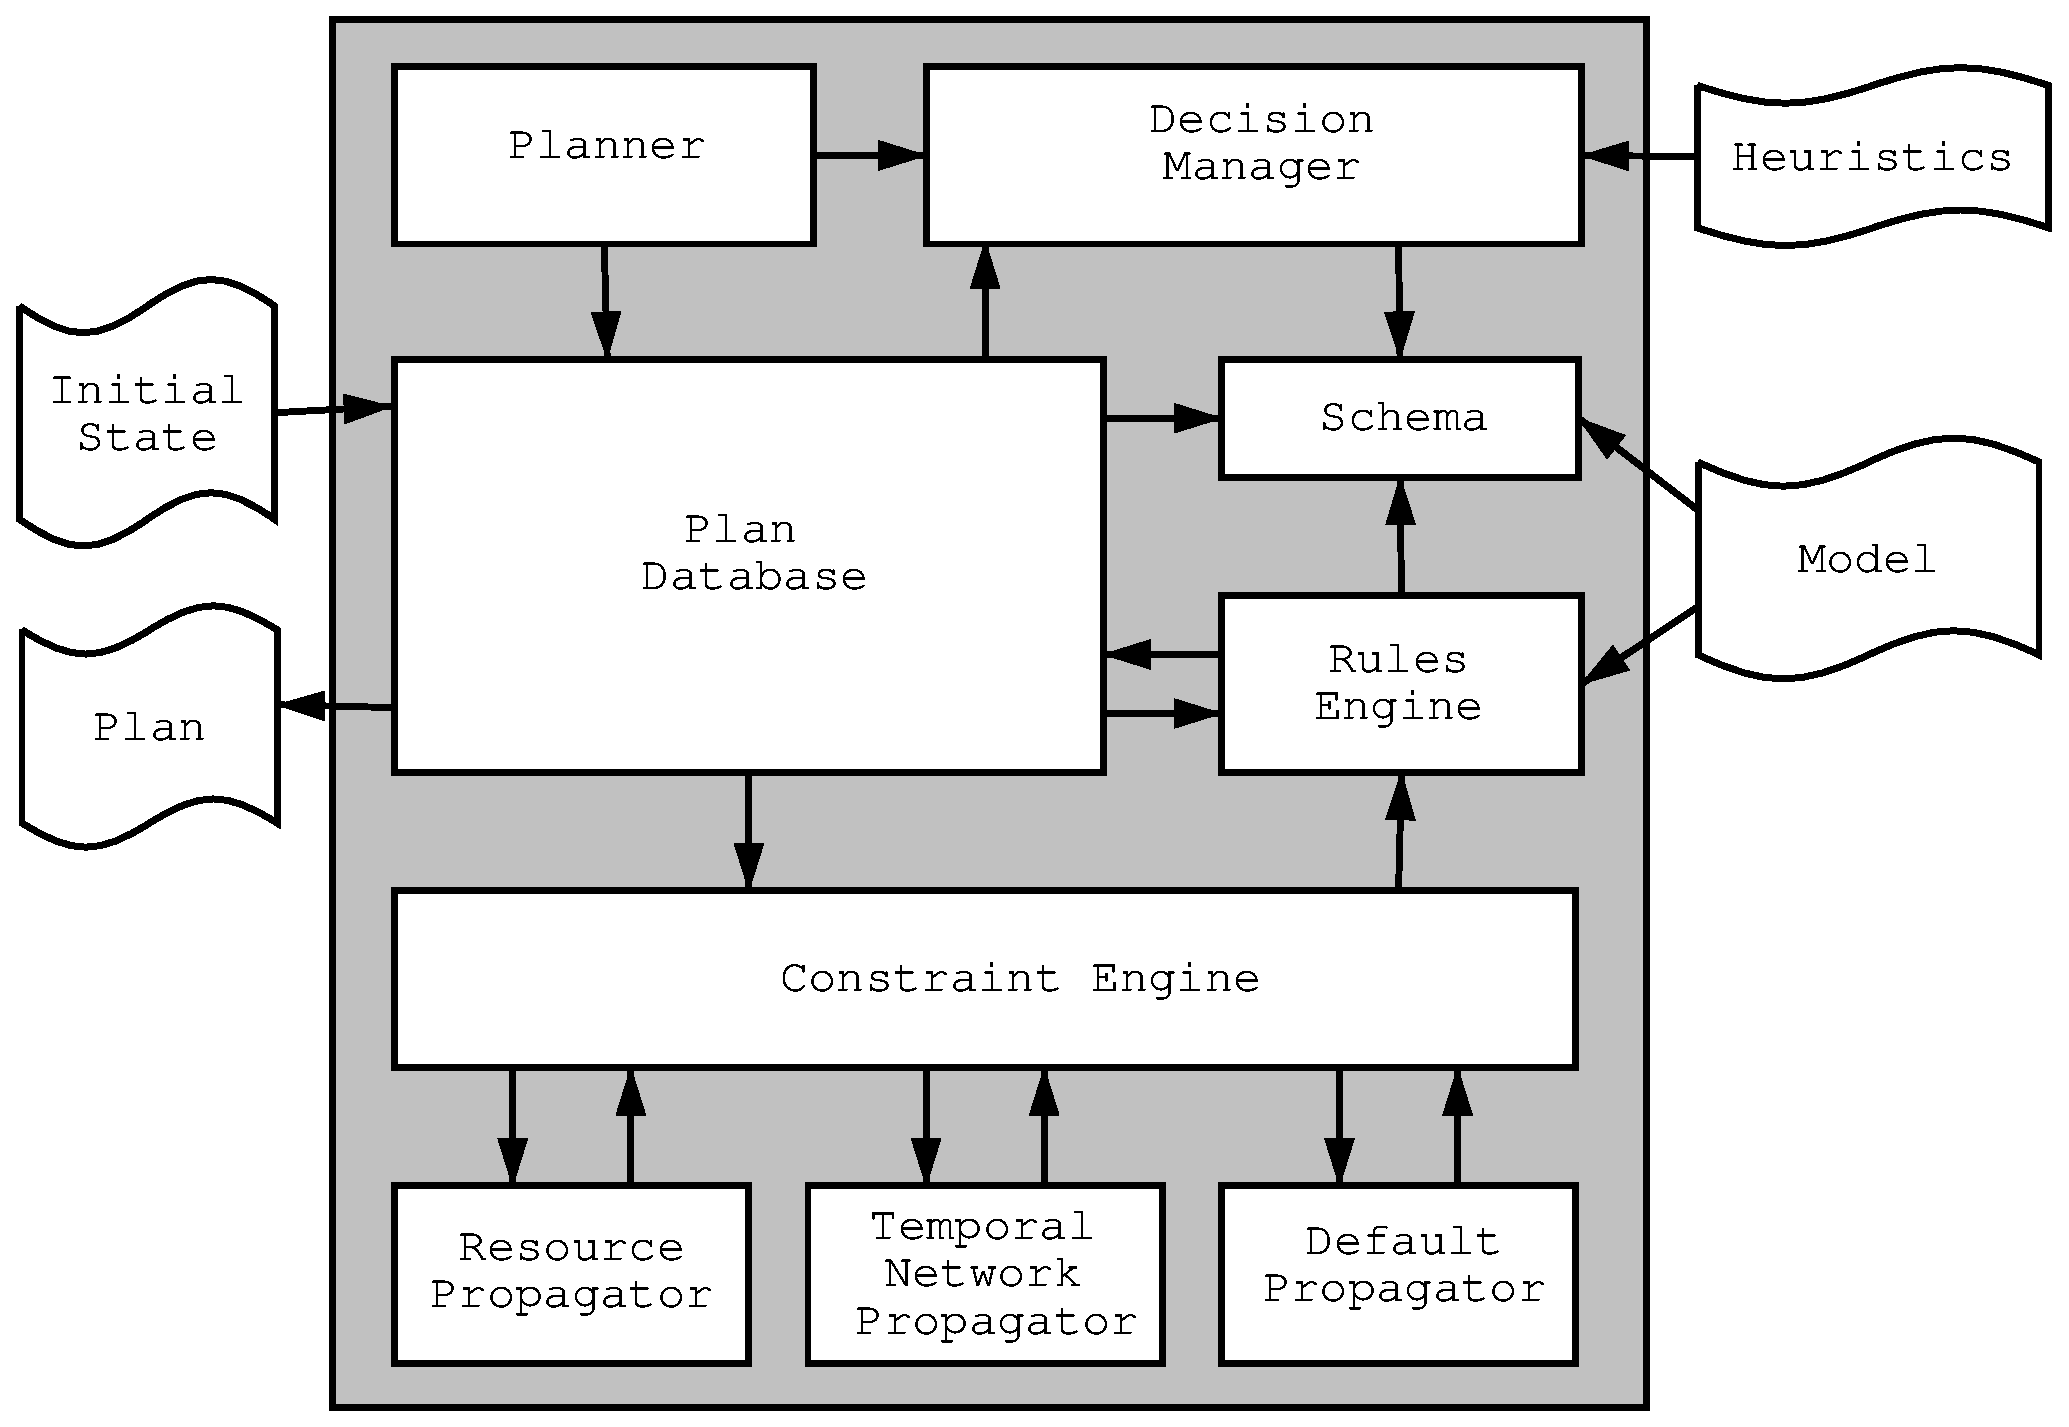
\epsfig{file=SystemDiagram.eps, width = 3.25in}
\caption{EUROPA System Architecture Diagram}
\label{SystemDiagram}
\end{figure}

Picture of overall architecture. Document each component at the level
of its main roles and responsibilities. This should be used as an
introduction to the API documentation. Ideally, we could directly
leverage that documentation.
\subsection{Plan Database}
\subsection{Constraint Engine}
\subsection{Temporal Network}
\subsection{Rules Engine}
\subsection{Resources}
\subsection{NDDL Parser and Compiler}
\subsection{Utilities}
\subsection{CBPlanner}
\subsection{Key use cases}


\begin{figure}[t]
\centering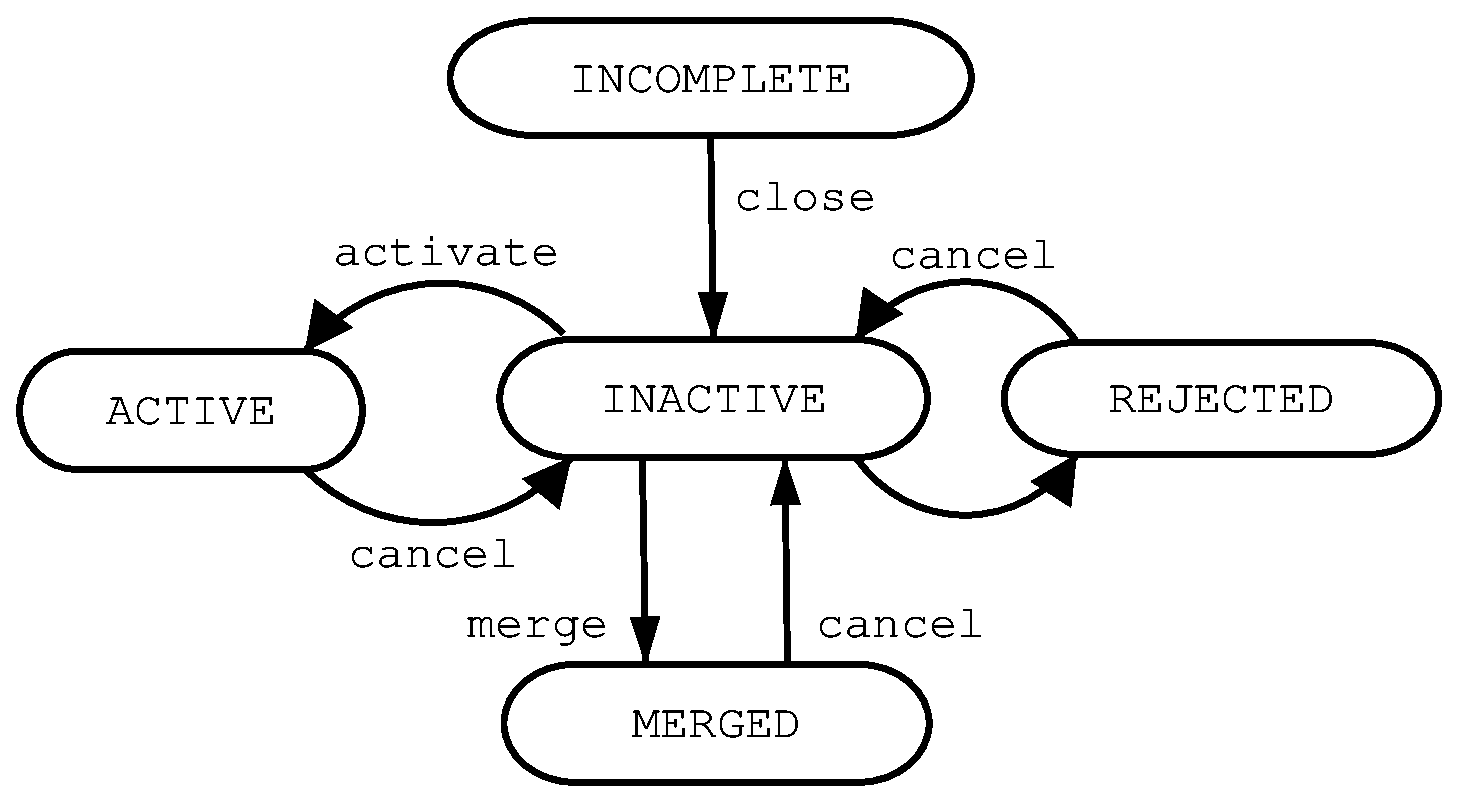
\epsfig{file=TokenStateModel.eps, width = 3.25in}
\caption{Token State Transition Diagram}
\label{TokenStateModel}
\end{figure}

Helps to understand the interaction among components. May want to use
a simple example model, possibly cut-down from k9.
\begin{enumerate}
\item Creating an Object
\item Token activation
\item Token deactivation
\item Constraining a Token
\item Freeing a Token
\item Binding a Variable
\item Freeing a Variable
\item Copying a plan database
\end{enumerate}

\section{Customization and Extension}
\subsection{Configuration and Assembly}
\subsection{Using and extending the CBPlanner}
\subsection{Custom constraints}
\subsection{Custom propagation}
\subsection{Building model specializations}
\subsection{Custom rule implementations}
\subsection{Specialized domains}
\subsection{External data integration}
\subsection{Listeners and Loggers}
\subsection{Integration to PlanWorks}

\section{Bibliography}

\section{Appendices}
\subsection{Appendix A: NDDL Language Reference}

class
predicate
int
float
string
enum
extends
concurrent
precedes
object
start
end
duration
state
time
new
goal
rejectable
activate
specify
constrain
close

\subsection{Appendix B: Temporal Relations}

In NDDL, two tokens can be constrained in several simple ways,
including with the following ``abbreviations'' for several commonly
used constraints.  In the examples, ``A'' and ``B'' are tokens.
``A.start'' is therefore the time at which token A starts; similarly,
``B.end'' is the time at which token B ends.

\begin{tabular}{ll}
NDDL syntax & Constraints created \\
\cline{1-2} \\
A after B; & B.end <= A.start \\
A any B; & (none) \\
A before B; & A.end <= B.start \\
A contained\_by B; & B.start <= A.start, A.end <= B.end \\
A contains B; & A.start <= B.start, B.end <= A.end \\
A contains\_end B; & A.start <= B.end, B.end <= A.end \\
A contains\_start B; & A.start <= B.start, B.start <= A.end \\
A ends B; & A.end = B.end \\
A ends\_after B; & B.end <= A.end \\
A ends\_after\_start B; & B.start <= A.end \\
A ends\_before B; & A.end <= B.end \\
A ends\_during B; & B.start <= A.end, A.end <= B.end \\
A equal B; & A.start = B.start, A.end = B.end \\
A meets B; & A.end = B.start \\
A met\_by B; & A.start = B.end \\
A paralleled\_by B; & B.start <= A.start, B.end <= A.end \\
A parallels B; & A.start <= B.start, A.end <= B.end \\
A starts B; & A.start = B.start \\
A starts\_after B; & B.start <= A.start \\
A starts\_before B; & A.start <= B.start \\
A starts\_before\_end B; & A.start <= B.end \\
A starts\_during B; & B.start <= A.start, A.start <= B.end \\
\end{tabular}

Here are the inverse relations.

\begin{tabular}{ll}
NDDL syntax & Inverse relation \\
\cline{1-2} \\
A after B; & A before B; \\
A any B; & A any B; \\
A before B; & A after B; \\
A contained\_by B; & A contains B; \\
A contains B; & A contained\_by B; \\
A contains\_end B; & A ends\_during B; \\
A contains\_start B; & A starts\_during B; \\
A ends B; & A ends B; \\
A ends\_after B; & A ends\_before B; \\
A ends\_after\_start B; & A starts\_before\_end B; \\
A ends\_before B; & A ends\_after B; \\
A ends\_during B; & A contains\_end B; \\
A equal B; & A equal B; \\
A meets B; & A met\_by B; \\
A met\_by B; & A meets B; \\
A paralleled\_by B; & A parallels B; \\
A parallels B; & A paralleled\_by B; \\
A starts B; & A starts B; \\
A starts\_after B; & A starts\_before B; \\
A starts\_before B; & A starts\_after B; \\
A starts\_before\_end B; & A ends\_after\_start B; \\
A starts\_during B; & A contains\_start B; \\
\end{tabular}

The names used for the relations as defined in James Allen's original
paper [] are:

\begin{tabular}{lll}
Allen Relation & Constraints & Equivalent Europa Relation \\
\cline{1-3} \\
A equals B (=) & A.start = B.start, A.end = B.end & A equal B \\
A precedes B (<) & A.end < B.start & A before [1 +Inf] B \\
A follows B (>) & A.start > B.end & A after [1 +Inf] B \\
A meets B (m) & A.end = B.start & A meets B \\
A inverse-meets B (im) & A.start = B.end & A met\_by B \\
A during B (d) & A.start > B.start, A.end < B.end & A contained\_by [1 +Inf] [1 +Inf] B \\
A inverse-during B (id) & A.start < B.start, A.end > B.end & A contains [1 +Inf] [1 +Inf] B \\
A starts B (s) & A.start = B.start, A.end < B.end & A parallels [0 0] [-Inf -1] B \\
A inverse-starts B (is) & A.start = B.start, A.end > B.end & A parallels [0 0] [1 +Inf] B \\
A finishes B (f) & A.start > B.start, A.end = B.end & A parallels [-Inf -1] [0 0] B \\
A inverse-finishes B (if) & A.start < B.start, A.end = B.end & A parallels [1 +Inf] [0 0] B \\
A overlaps B (o) & A.start < B.start, A.end > B.start, A.end < B.end & <unsupported as a single relation> \\
A inverse-overlaps B (io) & A.start < B.end, A.end > B.start, A.end > B.end & <unsupported as a single relation> \\
\end{tabular}

Note the explicit naming of nearly all of the inverse relations.
The exceptions are ``equals'' (its own inverse) and ``precedes'' and
``follows'', which are each other's inverse.

Note also the need for explicit bounds in most of the equivalencies
due to Europa's relations being based on, e.g., ``before or at the same
time'' rather than Allen's relations being strictly ``before'' and the
lack of explicit support for the last two Allen relations.  Europa
II's additional flexibility does allow them to be expressed, though
more verbosely, as the constraints themselves.  E.g.:

\begin{tabular}{ll}
Allen Relation & NDDL Constraints \\
\cline{1-2} \\
A overlaps B (o) & LessThan(A.start, B.start); LessThan(B.start, A.end); LessThan(A.end, B.end); \\
A inverse-overlaps B (io) & LessThan(A.start, B.end); LessThan(B.start, A.end); LessThan(B.end, A.end); \\
\end{tabular}

\subsection{Appendix C: Constraint Library Reference}
\subsection{Appendix D: Test Language Specification and Use}
\subsection{Appendix E: Coding Guidelines}

\begin{itemize}
\item[] General Practices
 \begin{itemize}
  \item	Ensure you declare variables and methods in their narrowest scope.
  \item	If you declare a static variable inside a non-static method, double check that the method should not be static and also double check that the variable should not be a member of the class.
  \item	We discourage writing code in header files unless needed for templates or proven performance.
  \item	Use STL classes and methods unless what you need is not provided.  Same goes for any other code.  Reuse as much as possible. 
 \end{itemize}

\item[] Pre-processing
 \begin{itemize}
  \item	Include system headers by using the angle bracket style. (\#include <stdio>)
  \item	Include user files by using the double quote style. (\#include "File.h")
  \item	Do not define your own pre-processor macros to control level of or presence of debugging output or error checks.
 \end{itemize}

\item[] Namespaces
 \begin{itemize}
  \item	Use the std:: prefix, or 'using namespace std;' when using STL.
  \item	Put Europa code in the Europa namespace.
 \end{itemize}

\item[] Global Constants
 \begin{itemize}
  \item	Use DEFINE\_GLOBAL\_CONSTANT and DECLARE\_GLOBAL\_CONSTANT for globals.
 \end{itemize}

\item[] Static Class Members
 \begin{itemize}
  \item	When handling static data, you must provide an automatic purge mechanism or provide an explicit purge method.
 \end{itemize}

\item[] Module Initialization and Termination
 \begin{itemize}
  \item	We should standardize method calls to initialization and termination methods.  Such as nddl initialization which cascades onto constraint engine initialization.
 \end{itemize}

\item[] Iterator Use
 \begin{itemize}	 
  \item	 Use const iterators unless you have to use a non-const iterator. 
  \item	 When using const iterators, use ++iterator rather than iterator++.
 \end{itemize}

\item[] Pointer References
 \begin{itemize}	
  \item	Direct pointer references are discouraged; use class Id instead.
  \item	When creating a reference, create an m\_id member that holds the id that gets constructed in the constructor initializer, in the destructor the m\_id should be removed.
  \item	When deleting references to ids call delete on the cast operator (e.g. delete (ConstrainedVariable *) ref).
 \end{itemize}

\item[] Magic Numbers
 \begin{itemize}      
  \item	Define an enumerated type to handle number references instead of using magic numbers.
 \end{itemize}

\item[] Classes
 \begin{itemize}
  \item	Capitalize names of classes.  When composing names for classes capitalize the first letter of each word.
  \item	Declare a virtual destructor.
 \end{itemize}

\item[] Pure Virtual Classes
 \begin{itemize}
  \item	Declare a protected constructor.
  \item	Declare all functions pure virtual.
 \end{itemize}

\item[] Methods
 \begin{itemize}
  \item	Declare a method const where possible.
  \item	Do not return bare pointers or non-const references.
  \item	If the caller can own a data structure that is to be populated in the callee, create the data structure in the caller and then pass it by reference as an argument.
  \item	Avoid copying of data structures where possible.
  \item	Declare non-primitive arguments as const references.
  \item	Return non-primitive values as const references.
 \end{itemize}

\item[] Error Checks
 \begin{itemize}
  \item	Use checkError to express pre-conditions.
  \item	Use checkError to express invariants.
  \item	Use checkError to express post-conditions.
  \item	Avoid using non-const functions in checkError tests.
  \item	Do not use assert.
  \item	Do not use Id::isValid outside of checkError.
  \item	Do not write "if (Test) checkError(...Check...);".  Write "checkError(!Test || ...Check...)".
 \end{itemize}

\item[] Debugging Output
 \begin{itemize}
  \item	Use the Europa debugging output management system.
  \item	Do not put debugging output into stdout or stderr.
 \end{itemize}

\item[] Documentation
 \begin{itemize}
  \item	Use doxygen style comments with the javadoc style keywords. (@brief, etc.)
  \item	Enforce emacs macros
  \item	Class descriptions, file descriptions, parameters, method, return values, errors  
  \item	Documentation is required for header files, recommended for implementation files
 \end{itemize}
\end{itemize}

\section{Acknowledgements}

This research was supported by NASA Ames Research Center and the NASA
Intelligent Systems program. 

\bibliography{user-guide}



\end{document}
